\documentclass{article}
\usepackage{tikz}
\usetikzlibrary{fadings,decorations.pathmorphing,decorations.text}
\definecolor{navyblue}{RGB}{0,0,128}
\usepackage{geometry}
\geometry{paperwidth=18cm,paperheight=9.5cm,top=2pt,left=0pt,right=0pt,bottom=0pt}
\pagestyle{empty}
\begin{document}
\centering
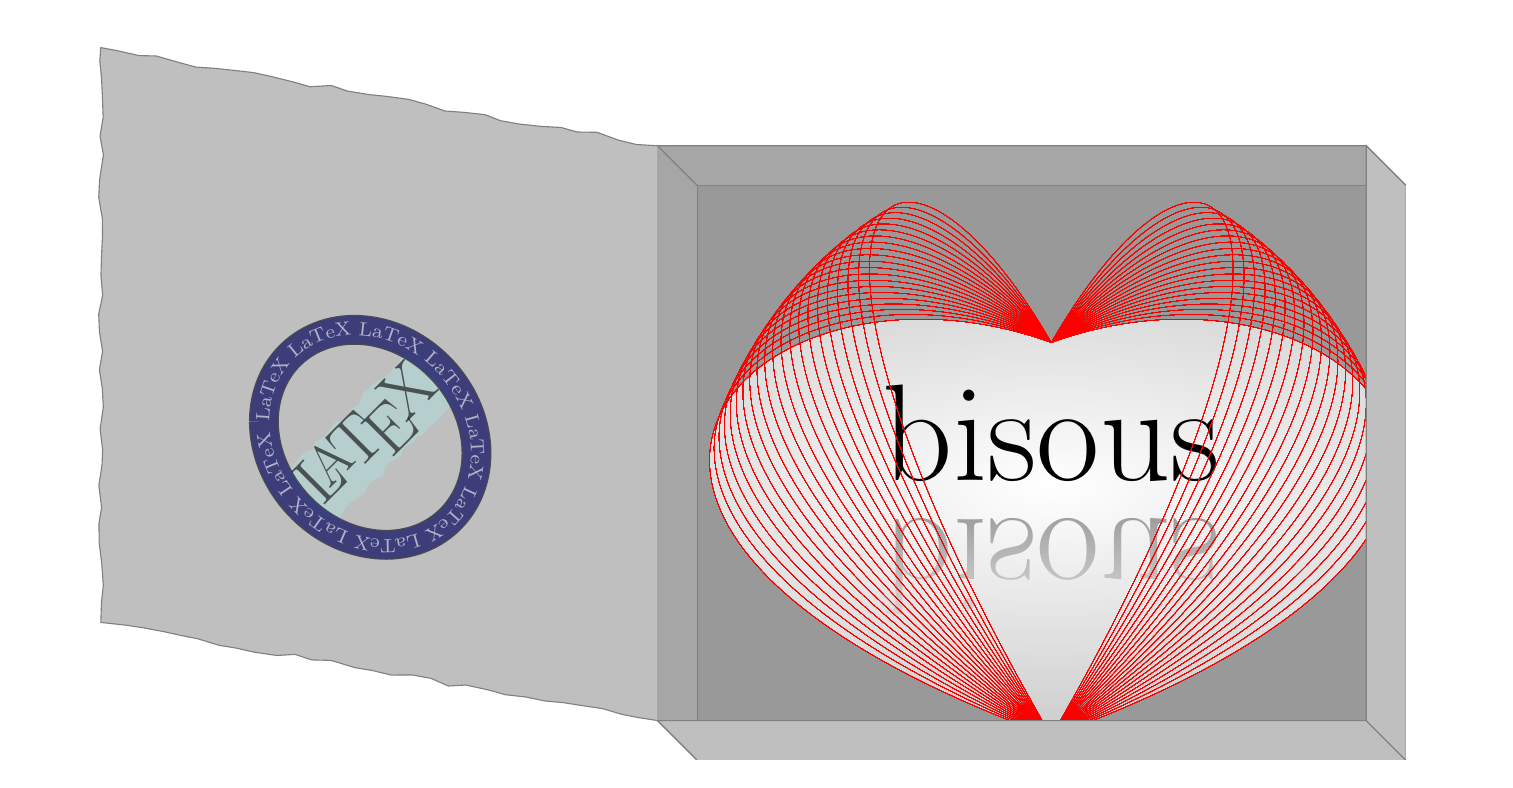
\begin{tikzpicture}
\clip(-13,-0.3) rectangle (5.5,9); 
\draw[gray,fill=gray!80] (-4.5,-0.3) rectangle (4.5,7);
\shade[shading=ball,inner color=white,outer color=black!20] (0,5) .. controls +(20:4) and (20:8)  .. (0,0)
							 (0,5) .. controls +(160:4) and (160:8) .. (0,0);
\def\nodeshadowed[#1]#2;{%
\node[scale=2,above,#1]{#2};
\node[scale=2,above,#1,yscale=-1,
scope fading=south,opacity=0.4]{#2};
}
\nodeshadowed[ at={(0,3)}]{ \Huge {bisous}};
\foreach \x in {20,22,...,60} \foreach \y in {160,158,...,120}
		{\draw[color=red,ultra thin] (0,5)..controls +(\x:4) and (\x:8).. (0,0)
 		(0,5)..controls +(\y:4) and (\y:8) .. (0,0);}
\draw[gray,fill=gray!70] (-4.5,-0.3)--++(-0.5,0.5) --++(0,7.3)--++(0.5,-0.5);
\draw[gray,fill=gray!50] (-4.5,-0.3)--++(-0.5,0.5) --++(9,0)--++(0.5,-0.5);
\draw[gray,fill=gray!70] (-4.5,7)--++(-0.5,0.5) --++(9,0)--++(0.5,-0.5);
\draw[gray,fill=gray!50] (4.5,-0.3)--++(-0.5,0.5) --++(0,7.3)--++(0.5,-0.5);
\draw[gray,fill=gray!50,
	decorate,decoration={random steps,segment length=7pt,amplitude=1pt}] 
	(-5,0.2) -- ++(170:7.18) -- ++(0,7.3)--++(-10:7.18);
\node(reference) at(-10,4){};
\draw[yslant=-0.15,opacity=0.6] (reference)+(1.35,0) node[inner ysep=1pt,decorate,decoration={random steps,segment length=3pt,amplitude=1pt},fill=teal!30,rotate=45,font=\Huge]{\LaTeX};
\draw[yslant=-0.15,opacity=0.6,double=navyblue!80,double distance=1em,
	postaction={decorate,decoration={raise=-2pt,text along path,text=|\scriptsize\color{white}|LaTeX LaTeX LaTeX LaTeX LaTeX LaTeX LaTeX LaTeX LaTeX LaTeX LaTeX LaTeX}}] 
	(reference) arc (180:-180:1.35cm);
\end{tikzpicture}
\end{document}
